%%%%%%%%% NEW SECTION: INTRODUCTION %%%%%%%%%

\section{Introduction}
The CRIMI (ChRIs $\&$ MIchelson) is an infrared Fourier transform spectrometer, made by Chris de Jonge, under supervision of Dr. Andrey Baryshev. The spectrometer is designed to be used in a vacuum, as water molecules and other abundant molecules in the atmosphere absorb large parts of the infrared spectrum.

The goal of this internship was to write software to guide the linear stage in the CRIMI to make measurements, design a graphical user interface for easy user access and do some data processing on the acquired data: fast Fourier transforms and windowing. As a result, I have written a program in Python that automatically takes a complete measurement with this spectrometer. The program takes scan length and stepsize, or equivalent resolution and maximum frequency, as input, and outputs the raw data in \verb!csv! format.

%Doe hier ook een plaatje van een FTS (kun je van WIKIPEDIA halen). doel van je stage was:
%aansturing van linear stage
%grafische user interface
%data processing (FFT algorithmes + windowing)
%Zet in deze introductie ook een formule en plaatje met spectrum en interferogram.
%\textbf{Verder is het goed om hier ook aan te geven hoe padlengte de resolutie bepaalt, en minimale stapgrootte de hoogste frequentie.}

\subsection{Fourier Transform}

Fourier transform spectrometers (FTS) work on the interference and Fourier principles. The spectrometer has a moveable part and stationary parts. In the case of figure~\ref{fig:fts}, a moving mirror provides a difference in distance travelled by the two beams of light created by the beamsplitter. By moving one mirror, the path length $l_1$ is made different from $l_2$, which produces an interference pattern when the light is recombined. This pattern is a cosine wave for each wavelength. Because of the range of wavelengths in the source, at different positions of the mirror, different wavelengths are attenuated.

\begin{figure}
 \begin{center}
  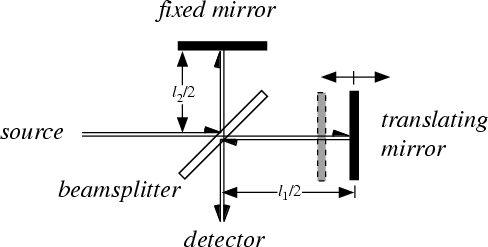
\includegraphics[width=0.8\textwidth]{figures/fts.png}
  \caption{A simple Fourier transform spectrometer (FTS). Path length differences are created by moving parts of the setup.  From \cite{wolf}.}
  \label{fig:fts}
 \end{center}
\end{figure}


With a Fourier transform the intensity for each position ($\delta$) is turned into the intensity for each wavenumber ($\tilde{\nu}$), because one is the inverse of the other: $\tilde{\nu} = \frac{1}{\delta}$, and from this the frequency $f$ can be computed: $\tilde{\nu}\cdot c=f$. $\delta$ and $\nu$ are together called a Fourier transform pair.

The Fourier transform of a function is the following formula:

\[
 F(\omega)=\int_{-\infty}^{\infty}f(t)e^{-i\omega t}dt,
\]
with $i$ the unit imaginary number. However because all wavelengths produce cosine waves, the total input is just a summation of cosines. Also we talk about position and wavenumber, so in this case the Fourier transform can be simplified to

\[
 F(\tilde{\nu}) = \int_{-\infty}^{\infty}f(\delta)\cos(2\pi\delta\tilde{\nu})d\delta,
\]

with $F(\tilde{\nu})$ the power of the source as a function of wavenumber or frequency, and $f(\delta)$ the power as a function of path length difference.

Because of this Fourier transform and $\tilde{\nu} = \frac{1}{\delta}$, a longer path length for the measurement causes a higher resolution, and a smaller stepsize gives a higher highest frequency.

In the software this computation is done by taking the fast Fourier transform, an algorithm which uses a list of equally spaced samples of some periodic function to compute the Fourier transform and its inverse. Therefore it is necessary to take measurements which are equally spaced, in this case in distance.

These kind of algorithms assume that the measured range is an integer multiple of periods, which can never be achieved for broadband measurements. To compensate for the errors introduced by this assumption, a windowing or apodization function can be added. This function smoothes out the measurements to zero at the edges of the range, which minimizes these effects. There are different windowing functions, which can all be used after the measurements have been made and before the Fourier transform is done. In this program only the Hann apodization function has been added, as it is easy to include use other windowing functions on the saved interferogram data.

\begin{figure}
 \begin{center}
  \subfloat[The measured interferogram.]{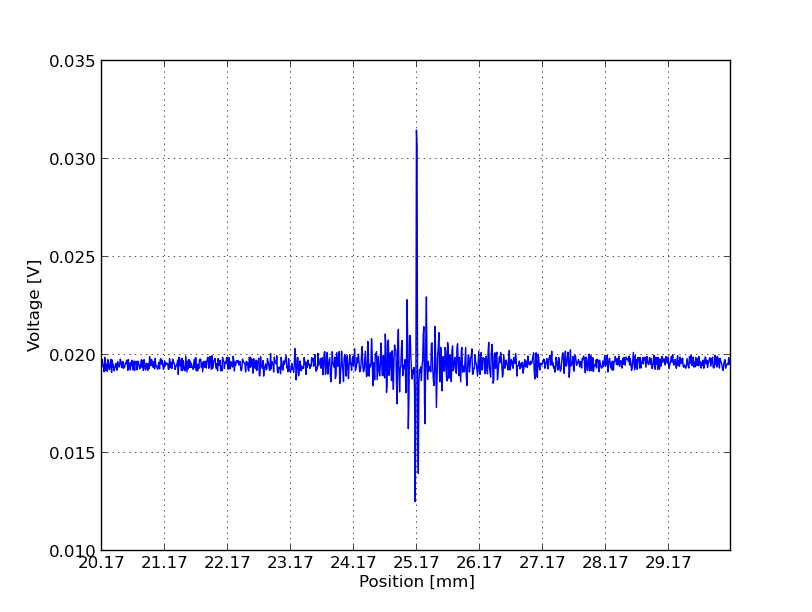
\includegraphics[width = 0.47\textwidth]{figures/interferogramforreport.png}}
  \quad
  \subfloat[The spectrum.]{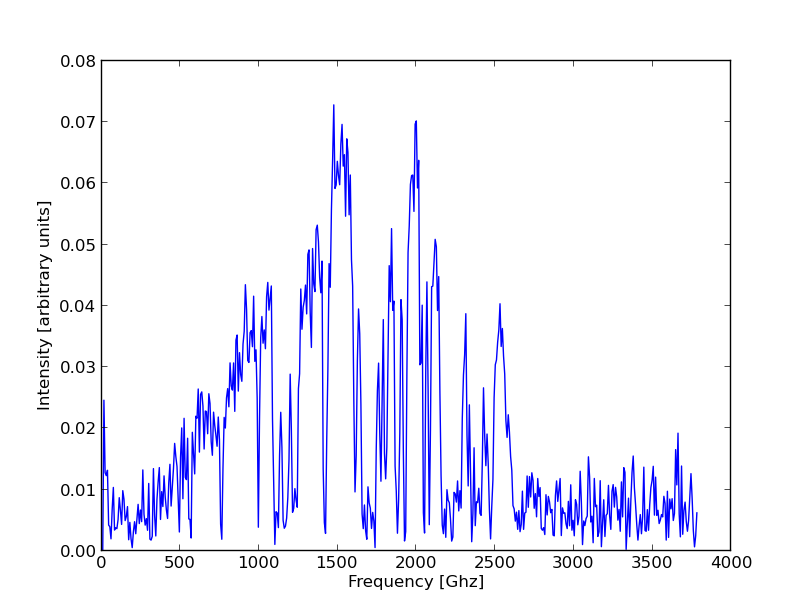
\includegraphics[width = 0.47\textwidth]{figures/fourierplotforreport.png}}
  \caption{The Fourier transform of an interferogram gives the spectrum.}
  \label{fig:fouriertransform}
 \end{center}
\end{figure}

\subsection{Hardware}

The spectrometer needs a few devices to function (see figure \ref{fig:hardware}). The controller to move the stage in is the PI C867.160 controller. The lock in amplifier in use is the SR510. A third device is needed to be able to communicate with the lock in amplifier from any computer: a GPIB-Ethernet adapter. This device counteracts the need for a special GPIB circuit card in the computer. All three are hardcoded into the software. This means unfortunately that the software does not automatically work with e.g. the SR530 lock in amplifier, or with a direct GPIB connection to the computer.

The test setup used a helium-cooled bolometer to actually measure the power of the radiation. This report will not deal any further with the measuring device, as the software is independent of that.


\begin{figure}[h!tb]
	\begin{center}
		\subfloat[The controller for the stage from PI.]{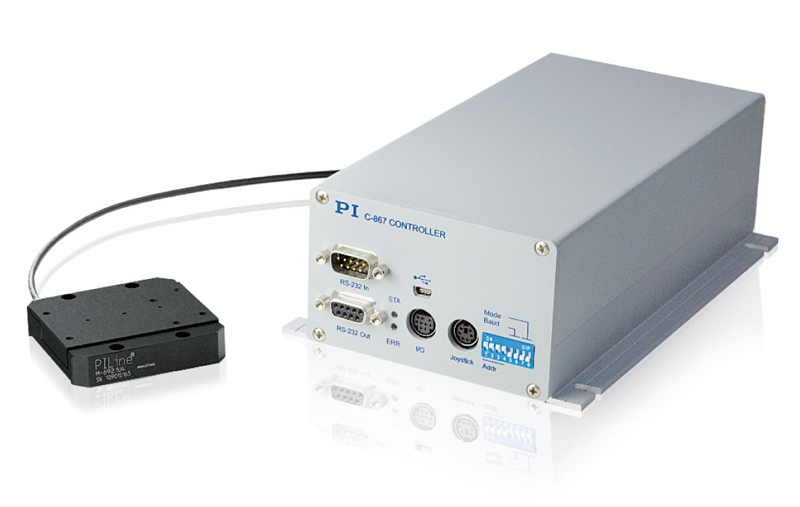
\includegraphics[width = 0.45\textwidth]{figures/pi_c867_160.jpg}}
		\qquad
		\subfloat[The SR510 lock in amplifier.]{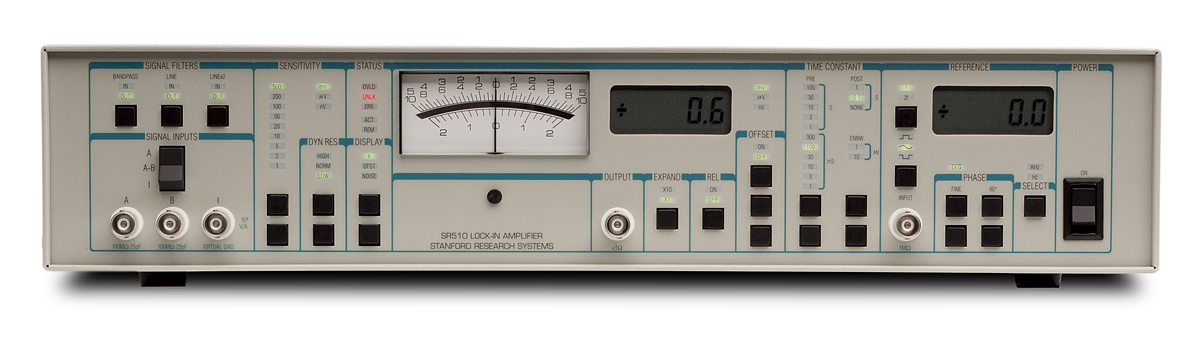
\includegraphics[width = 0.45\textwidth]{figures/SR510_FPlg.jpg}}
		\qquad
		\subfloat[The GPIB-Ethernet Controller.]{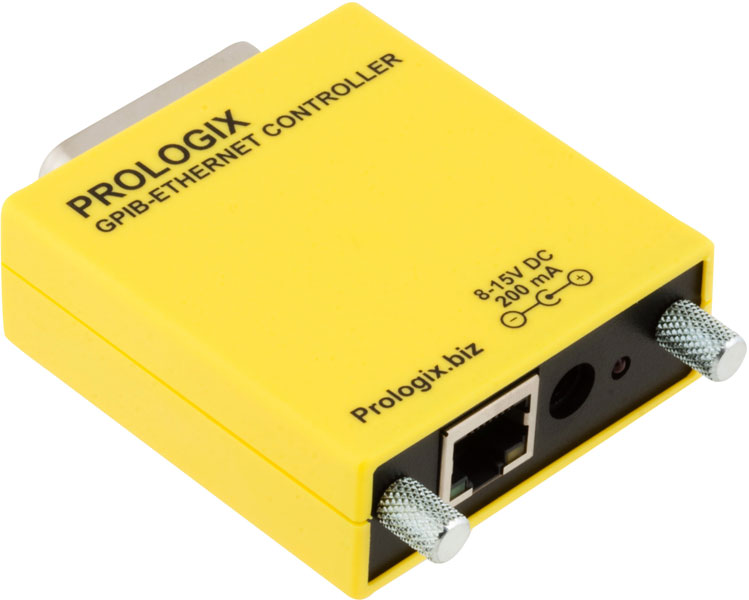
\includegraphics[width = 0.4\textwidth]{figures/GPIB-Ethernet-back.jpg}}
		\caption{The hardware. Pictures from \cite{PI}, \cite{SR}, and \cite{prologix}.}
		\label{fig:hardware}
	\end{center}
\end{figure}

It is important to mention that on the SR510 the DIP-switches need to be in a different configuration than the `example' configuration as mentioned in its manual on page 7. For fast readout, SW1 switch 6 should be in the `up' position instead of in the `down' position, to suppress echoing over the RS232 connection (which is unconnected in this setup). The SW2 switches are not of importance in this setup, as no RS232 connection is used. See figure~\ref{fig:SR510_back} for the location of this switch.

\begin{figure}[h!tb]
 \begin{center}
  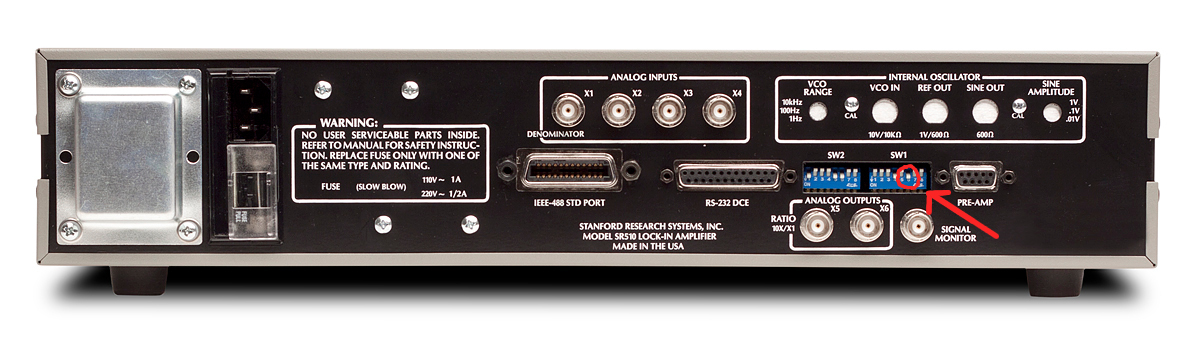
\includegraphics[width=\textwidth]{figures/SR510_Rear_circle.jpg}
  \caption{The back plate of the SR510 lock in amplifier. Encircled is SW1 switch 6. For fast performance, this switch should be in the `up' position. Picture from \cite{SR}.}
  \label{fig:SR510_back}
 \end{center}
\end{figure}


The software is written for Windows, because almost all the computers at SRON make use of Windows. This is hardcoded, because only the COM-ports (serial ports) are coded in.

\subsection{Python}
Python is an interpreted, interactive, object-oriented programming language \cite{python}. It is open source and free, and easy to learn. Python runs on Windows, Linux/Unix and Mac OS X. It has an active community that contributes a large number of libraries for various tasks, e.g. numerical mathematics and hardware interfacing.

Python has the distinct advantage over programming languages such as LabVIEW that it is backwards compatible. Old code written in previous versions is in many cases still executable in newer Python versions, and as the files are plain text, it will be always readable in any editor. So even when old code cannot be executed anymore, it can still be modified to comply with newer standards.

This software is written in Python version 2.7. The extra (non-native) packages needed for the program are \verb!PySerial! to open a serial port for the PI-controller and \verb!wxPython! to make the GUI. For this last task \verb!wxFormbuilder!, an open source GUI designer which emits Python code, was also used. The other imported packages are part of the core Python distribution.
